\chapter{Pruebas de Campo}

En este capitulo, se adjuntarán unos vídeos comprobando el funcionamiento del robot.

\begin{enumerate}
\item En el primer vídeo, después de haber realizado la soldadura de los motores y comprobado que existe conectividad, se verifica que su funcionamiento es el adecuado.
 
https://www.youtube.com/watch?v=pck8Bpla-5w
 
 \begin{figure} [hbtp]
  \begin{center}
    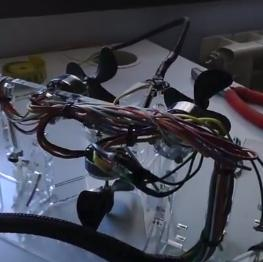
\includegraphics[width=7cm]{img/cap5/motores}
  \end{center}
  \caption{Prueba de motores}
  \label{fig:motores}
 \end{figure}

\item Una vez montado el robot, antes de llevarlo al exterior, se comprueba que es estanco y que el hardware no sufre ningún daño, para este proceso, llenamos la bañera de agua e introducimos el robot.
 
También se comprueba que funcionan todas las aplicaciones instaladas y que puede permanecer más de 6 horas bajo el agua sin incidentes.

https://www.youtube.com/watch?v=jqZOBc\_-mvU
\newpage
 \begin{figure} [hbtp]
  \begin{center}
    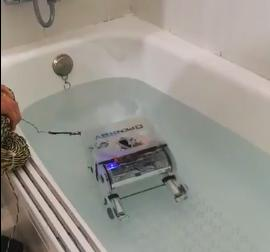
\includegraphics[width=7cm]{img/cap5/banera}
  \end{center}
  \caption{Prueba de funcionamiento en la bañera}
  \label{fig:banera}
 \end{figure}
 
\item Una vez comprobados los dos apatados anteriores, es momento de comprobar su funcionamiento en un entorno más hostil, para ello, nos hemos dirigido a un lago.
 
Antes de sumergirlo, comprobaremos que todo funciona correctamente y que no se necesita internet para interactuar con el robot.

https://www.youtube.com/watch?v=0LhODkpdkcw

 \begin{figure} [hbtp]
  \begin{center}
    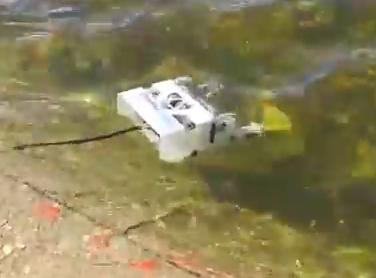
\includegraphics[width=7cm]{img/cap5/lago1}
  \end{center}
  \caption{Prueba de funcionamiento en el lago}
  \label{fig:lago}
 \end{figure}
 

\newpage
\item En este video, se comprueba que el robot puede navegar por el lago sin ningún problema.
 
https://www.youtube.com/watch?v=KLFG9klwu\_Q
 
 \begin{figure} [hbtp]
  \begin{center}
    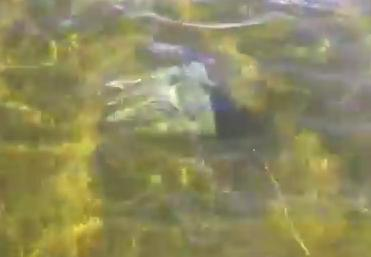
\includegraphics[width=7cm]{img/cap5/navegacion}
  \end{center}
  \caption{Prueba de navegación en el lago}
  \label{fig:navegacion}
 \end{figure}

\item Se realiza una prueba de emersión para comprobar que el robot puede volver a la superficie sin problemas.

https://www.youtube.com/watch?v=Q6qG2w9rGW0

 \begin{figure} [hbtp]
  \begin{center}
    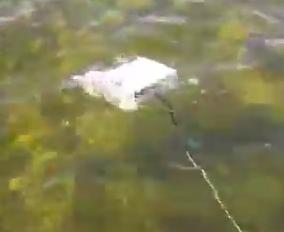
\includegraphics[width=7cm]{img/cap5/emersion}
  \end{center}
  \caption{Prueba de emersión del lago}
  \label{fig:emersion}
 \end{figure}

\newpage
\item En el último video, vemos gracias a la web, todo lo que el robot está visualizando en el fondo del lago.
 
https://www.youtube.com/watch?v=svbzpc0WSwE
 
 \begin{figure} [hbtp]
  \begin{center}
    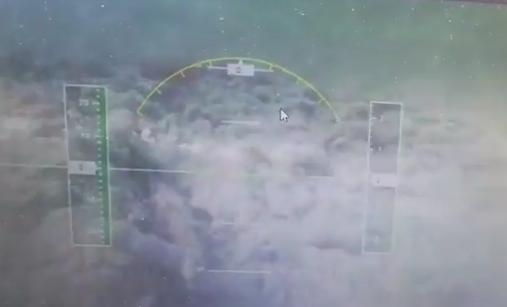
\includegraphics[width=7cm]{img/cap5/web}
  \end{center}
  \caption{Prueba de visualización del lago en la web}
  \label{fig:web}
 \end{figure} 


\end{enumerate}